\chapter{Experimentos}\label{cap.experimentos}
\hspace{1cm} En este capítulo se describen los experimentos realizados para validar el prototipo final, para comprobar el correcto funcionamiento del algoritmo completo y llegar a una solución final tras depurar mientras se desarrollaba. Para ello se ha dividido el código en tres partes a analizar: la primera parte, se ha evaluado la calidad del controlador, es decir, el error que comente el piloto al realizar una ruta predefinida; la segunda parte, se ha comprobado la calidad de autolocalización, es decir, se ha realizado una ruta teleoperada para ver los errores de posición de la aplicación y por último, se ha validado el error final de la aplicación con todos los componentes funcionando a la vez.

\hspace{1cm} Dada la complejidad de los experimentos, estos se han llevado a cabo dentro del entorno de simulación Gazebo. El plugin para la simulación del comportamiento del drone, así como el modelo necesario para la renderización del vehículo y sus sensores están incluidos en JdeRobot. Pero para evaluar correctamente los diferentes experimentos se han creado una serie de mundos en 3D, los cuales cuentan con espacios abiertos, espacios cerrados, balizas cuarteadas y AprilTags con sus correspondientes texturas. Los mundos creados se han integrado en los repositorios oficiales de JdeRobot bajo los nombres de \textit{ArDrone1}, \textit{ArDrone2} y \textit{ArDrone3}.

\hspace{1cm} Tanto para el cálculo de trayectorias, como para el cálculo de errores de distancia y de tiempos de ruta, se ha hecho uso del programa Matlab, el cual nos ha facilitado todos los procesos de cálculo. En la Figura \ref{fig:Mundo Gazebo.} se puede observar el mundo ArDrones1, que fue el primero que creamos y el máss representativo ya que se puede observar una posible aplicación de reconocimiento de un casa mediante el dron completamente automatizado. Cunetas con las balizas cuarteadas de despegue y aterrizaje, con 23 AprilTags para la autolocalización y con una casa a la cual tiene que darle una vuelta.

\begin{figure}[H]
	\begin{center}
		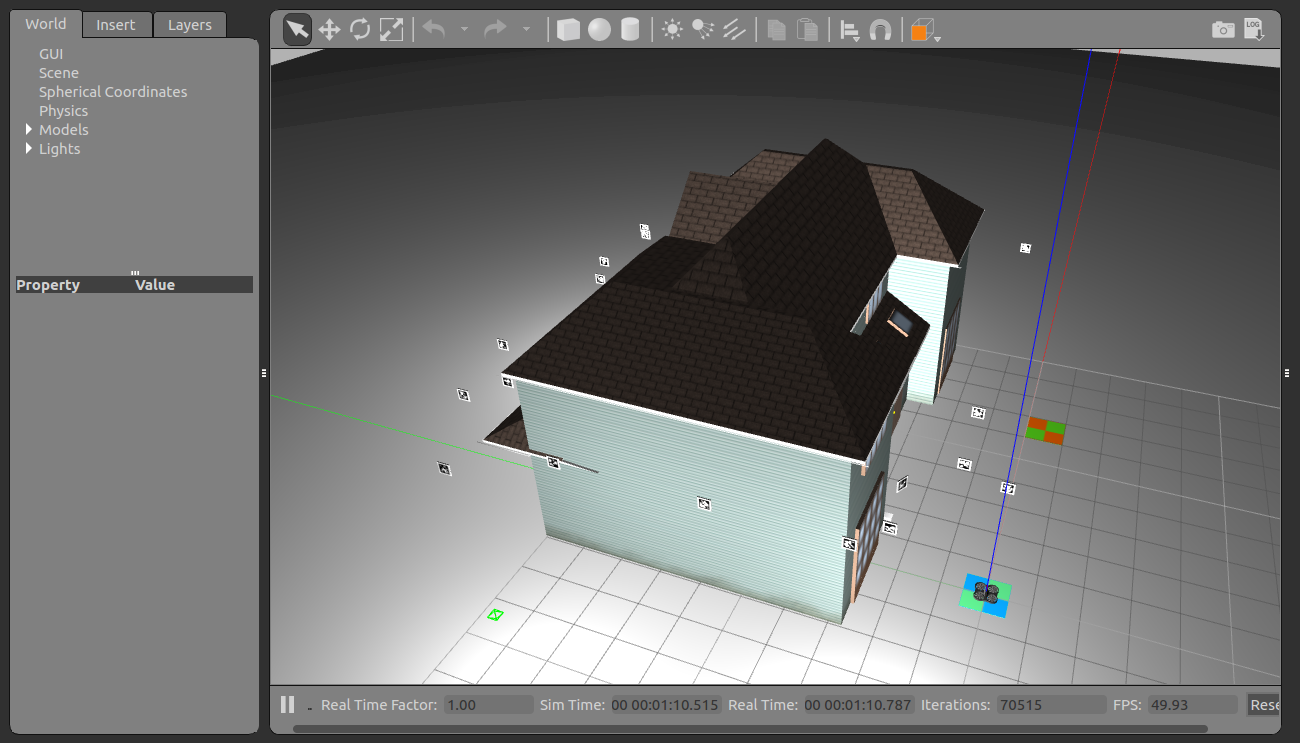
\includegraphics[width=1\textwidth]{imag/IMG28.png}
				\caption{Mundo Gazebo ArDones1.}
		\label{fig:Mundo Gazebo.}	
	\end{center}
\end{figure}


\section{Pruebas unitarias Autolocalización}
\hspace{1cm} Para evaluar el comportamiento de la nueva aplicación de JdeRobot, Slam-Visualmarkers, que se encarga de la autolocalización del drone, se aisló completamente de la parte de pilotaje. Para ello lo que se hizo fue teledirigir el drone dentro de un mundo de balizas el cual permitiese a la aplicación funcionar correctamente viendo al menos una AprilTag en toda la ruta. Una vez terminada la ruta se comparó la posición real entregada por el simulador $P_{0}$ con la posición estimada por el componente $P_{A} $. Dado que ambas estregan tanto posición (x y z) como dirección (Pitch Roll Yaw) se realizó un cálculo de error de posición mediante la distancia euclídea: 
\[ E_{p} = \sqrt{(P_{Ax}-P_{0x})^{2}+(P_{Ay}-P_{0y})^{2}+(P_{Az}-P_{0z})^{2}}\]
y lo que hemos definido como el error angular:    
\[ E_{a} = \sqrt{(P_{AP}-P_{0P})^{2}+(P_{AR}-P_{0R})^{2}+(P_{AY}-P_{0Y})^{2}}\]

\begin{figure}[H]
	\begin{center}
		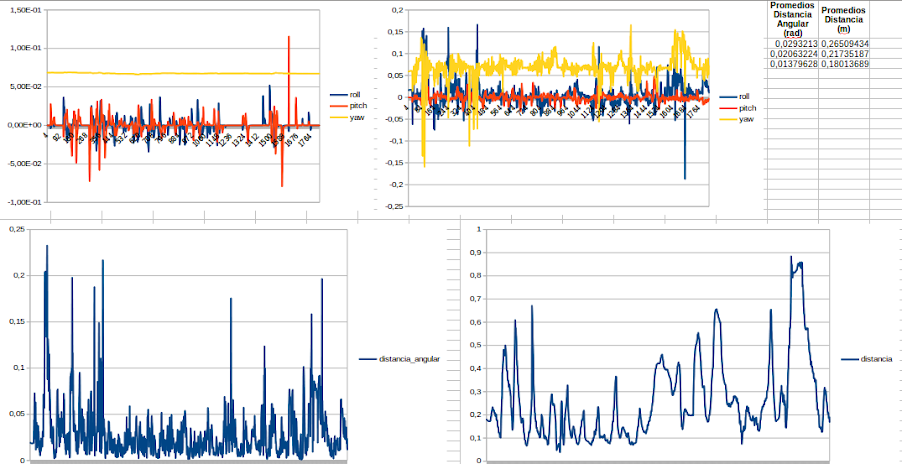
\includegraphics[width=1\textwidth]{imag/IMG36.png}
				\caption{Cálculo de errores de distancia y de ángulos}
		\label{fig:Error de distancia y de giro.}	
	\end{center}
\end{figure}

\hspace{1cm} Con la aplicación de las fórmulas anteriores se pueden obtener las gráficas de la figura \ref{fig:Error de distancia y de giro.}. En las gráficas superiores se ve la diferencia entre los tres ángulos pitch, roll y yaw del drone real (izquierda) con los calculados por la aplicación de Slam-VisualMarkers (derecha). Comparando visualmente las gráficas parece que el error sea elevado pero una vez analizados numéricamente los datos y calculando los errores con la fórmula anterior y representándolos en la gráfica inferior izquierda se ve como el error angular medio es de 0.0293rad lo que equivale a 1.679 grados lo que es un error muy pequeño, el error angular máximo es de 0.2329rad que son 13.344 grados. Por último. la gráfica inferior derecha nos muestra los errores de distancia euclídea entre la ruta realizada realmente con la posición que se calculaba con Slam-VisualMarkers, esta nos da que el error medio de distancia euclídea es de 0.2651m y el error máximo de distancia euclídea es de 0.8856m, con el cálculo de estos números y teniendo en cuenta que los errores máximos se producen cuando el drone solo ve una baliza y esta está alejada son cifras bastante razonables.

\begin{figure}[H]
	\begin{center}
		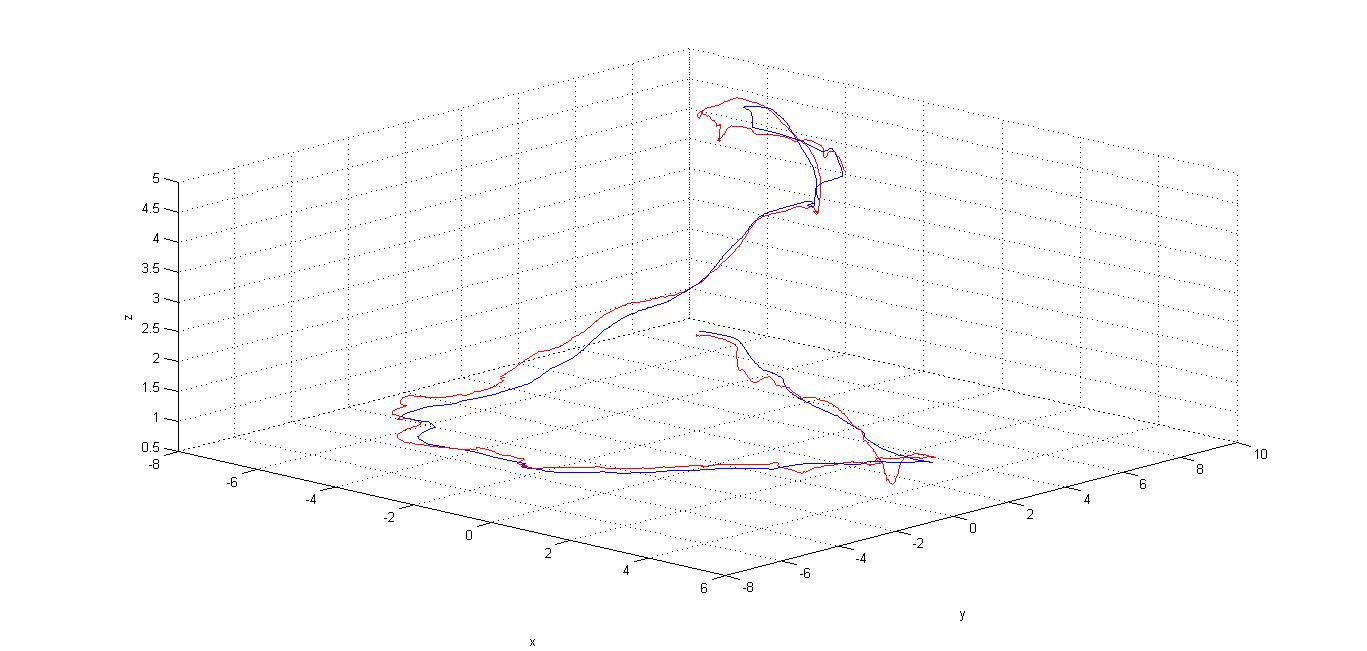
\includegraphics[width=1\textwidth]{imag/IMG48.jpg}
				\caption{Cálculo de posición de Slam-VisualMarkers}
		\label{fig:Comparativa Slam-Visualmarkers.}	
	\end{center}
\end{figure}

\hspace{1cm} Una vez realizados los cálculos del error se comprobó como cuando el componente pierde de vista las AprilTags los errores de posicionamiento aumentan considerablemente como se puede observar en la imagen \ref{fig:Comparativa Slam-Visualmarkers.}. Para evitar esto se habló con el desarrollador de la aplicación y se crearon una serie de  marcadores dentro del nuevo componente en ROS los cuales nos indicaban el número de balizas que se estaban viendo, con esto se pudo crear una nueva función que permite que cuando el drone no este viendo ninguna baliza no siga la ruta, sino que gire sobre sí mismo realizando círculos, cada vez mayores, sobre el último punto donde encontró la baliza, para así poder volver a encontrarla y posicionarse correctamente. Esto nos ayudó a que el drone no se perdiese de la ruta y siguiese moviéndose cuando no encontraba ninguna baliza, ya que ahora si da tres vueltas y seguía sin encontrar ninguna baliza, el drone aterriza. Con esta nueva función mejoramos la integridad de la aplicación y nos aseguramos de que el cuadricóptero no se aleje excesivamente de la ruta definida, preparándolo para los experimentos reales.

\section{Pruebas unitarias Pilotaje}
\hspace{1cm} Una vez comprendido el funcionamiento del drone con las practicas iniciales de \textit{JdeRobot Academy} empezamos a crear el piloto que permitiera al drone seguir rutas. El primer piloto se encargaba de seguir únicamente puntos de paso, es decir tan solo variaría su velocidad lineal. Los primeros experimentos mostraban como el piloto se acercaba correctamente al punto, pero a la hora de la aproximación final no lograba alcanzarlo, por lo que se tuvieron que realizar varias correcciones tanto de velocidades máximas en los ejes x e y, como de variaciones de velocidad según la cercanía al siguiente punto. Una vez conseguido todo esto se volvieron a ajustar los parámetros de velocidades máximas, esta vez en los tres ejes para conseguir que el error en una ruta por puntos nunca superase los 10cm. Para ello se tuvo que sacrificar la velocidad máxima cuando el drone se acercaba al siguiente punto, pero aun así, la velocidad media del drone continuaba siendo el 0.82 de la máxima. En la siguiente imagen se puede ver una ruta por puntos compleja (en verde) y como ajustando la velocidad cercana a los puntos, la ruta final del drone es más exacta (rojo) que permitiéndole una velocidad máxima mayor (azul). Por tanto, podremos elegir si queremos que realice la ruta con mayor rapidez o con una mayor exactitud.

\begin{figure}[H]
	\begin{center}
		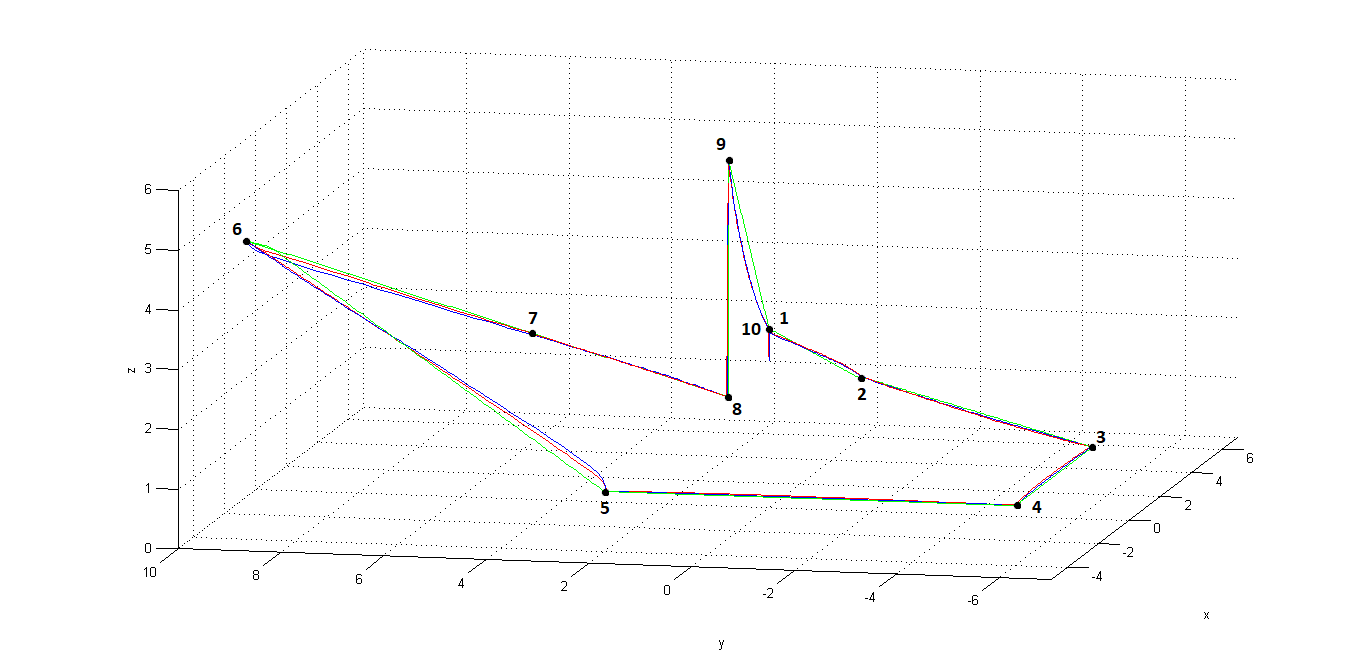
\includegraphics[width=1.0\textwidth]{imag/IMG47.png}
				\caption{Error asociado al pilotaje.}
		\label{fig:Error asociado al pilotaje.}	
	\end{center}
\end{figure}

\hspace{1cm} Después de validar el correcto funcionamiento del piloto por puntos se observó que este piloto solo sería valido para ciertas situaciones concretas por lo que se desarrolló un segundo piloto, el piloto por trayectorias, este piloto es más complejo ya que tiene variaciones de velocidad lineal y angular (en el ángulo de \textit{yaw}), al introducir giros el sistema presentaba comportamientos muy inestables. Para solucionar este comportamiento se realizó un estudio de relaciones de velocidades y se observó que el rango de velocidades para el funcionamiento estable del sistema de navegación era de [0.3-3.2]m/s. Del mismo modo, los valores de ganancia de giro debían estar comprendidos entre el rango [0.14-0.36]. Esta ganancia de giro era muy importante ya que valores muy altos significaban comportamientos inestables y valores muy bajos no permitían ajustar el giro de forma correcta. 

\hspace{1cm} A continuación se muestran diferentes ejemplos de rutas sencillas y complejas, en los cuales se ha comparado con pilotos anteriores de trayectorias para observar su mejora tanto de errores de distancias a la ruta como de tiempo de realización de rutas. En verde se muestra la ruta a seguir que es la que se le introduce al programa, en azul se ve la ruta que realiza el piloto antiguo y en rojo se muestra la ruta que realiza nuestro piloto.

\begin{figure}[H]
	\begin{center}
		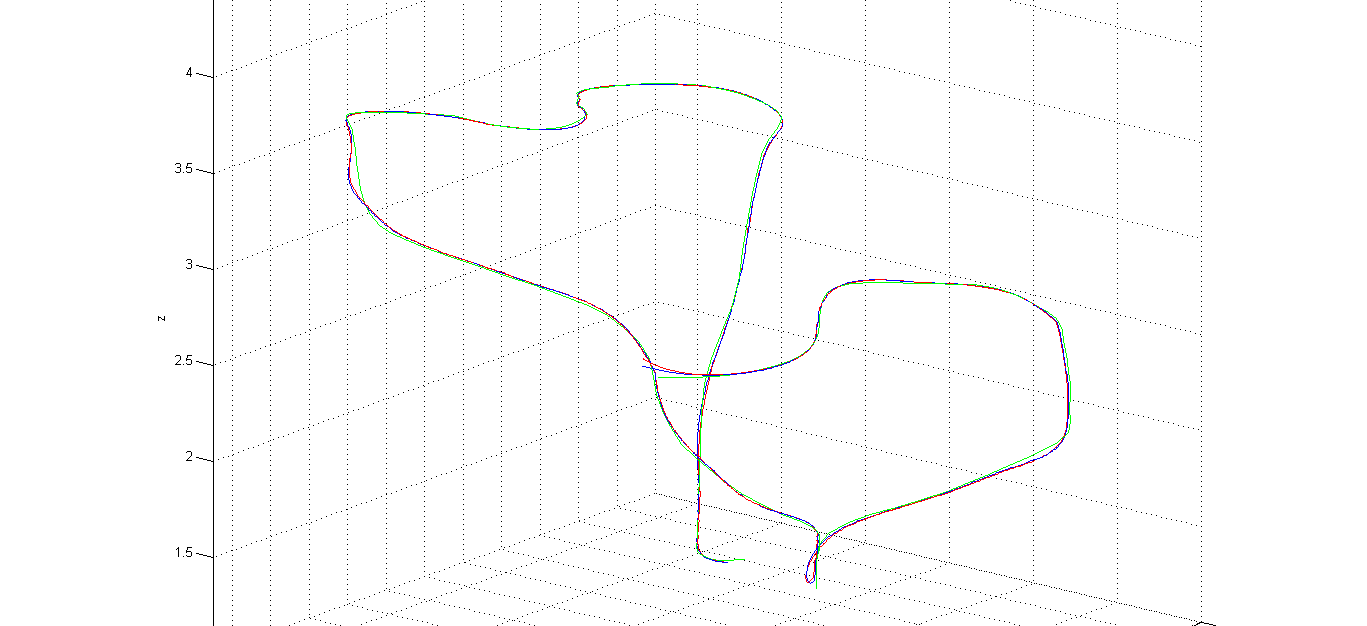
\includegraphics[width=1.0\textwidth]{imag/IMG40.png}
				\caption{Ruta sencilla en el pilotaje por trayectorias.}
		\label{fig:Ruta sencilla en trayectoria.}	
	\end{center}
\end{figure}

\begin{figure}[H]
 \centering
  \subfloat[Piloto Nuevo]{
   \label{f:Piloto Nuevo}
    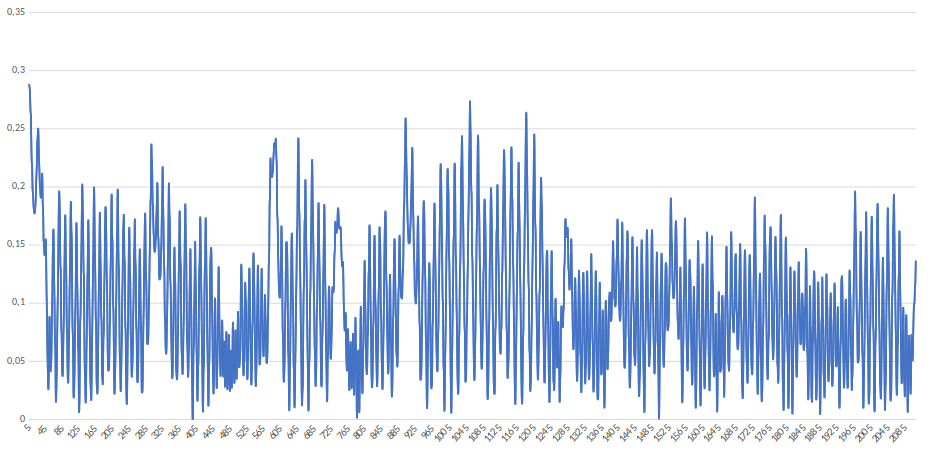
\includegraphics[width=0.5\textwidth]{imag/IMG45.png}}
  \subfloat[Piloto Antiguo]{
   \label{f:Piloto Antiguo}
    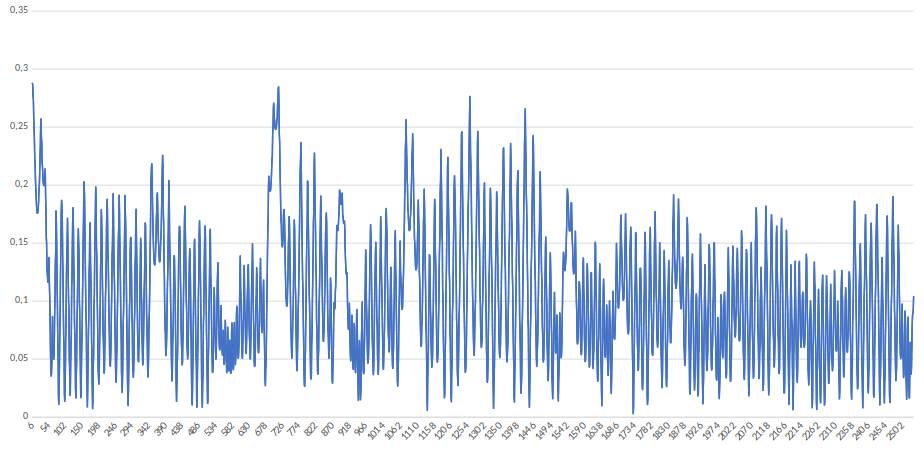
\includegraphics[width=0.5\textwidth]{imag/IMG46.png}} 
 \caption{Comparación del error entre ambos pilotos en ruta sencilla.}
 \label{f:Comparativa del error sencilla.}
\end{figure} 

\hspace{1cm} En la imagen \ref{fig:Ruta sencilla en trayectoria.} se puede observar como ambos pilotos son muy exactos a la hora de realizar las trayectorias deseadas que no cuentan con cambios de dirección muy bruscos ni con curvas muy cerradas, sobre todo en las partes rectas de las mismas donde se ve como el ajuste es prácticamente perfecto. En cuanto a las partes más difíciles como las curvas algo cerradas o los cambios bruscos de posición se observa en las gráficas \ref{f:Comparativa del error sencilla.} donde calculando el error obtenemos que el error de distancia media en nuestro piloto es de 0.1023m con un error máximo en ruta de 0.276m en cambio el piloto antiguo tiene un error medio de 0.1026m y un error máximo de 0.285m. Este error no crea una diferenciación demasiado grande en cuanto al piloto nuevo y al piloto antiguo en rutas sencillas, pero si nos centramos en el tiempo en que realizan la ruta el piloto nuevo tarda 188.72 segundos mientras que el antiguo utilizaba 253.35 segundos lo que supone una reducción del 25,51\% del tiempo en vuelo algo muy importante debido a la corta autonomía de los drones.

\begin{figure}[H]
	\begin{center}
		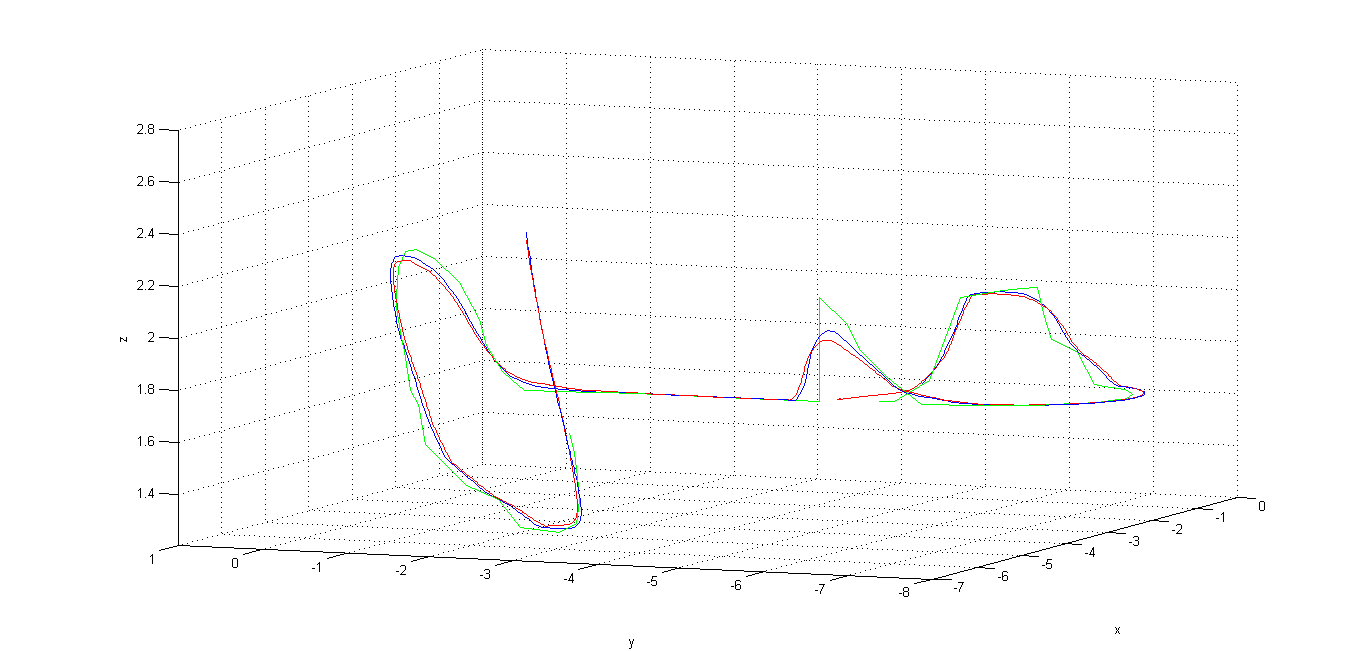
\includegraphics[width=1\textwidth]{imag/IMG41.png}
				\caption{Ruta compleja en el pilotaje por trayectorias.}
		\label{fig:Ruta compleja en trayectoria.}	
	\end{center}
\end{figure}

\begin{figure}[H]
 \centering
  \subfloat[Piloto Nuevo]{
   \label{f:Piloto Nuevo}
    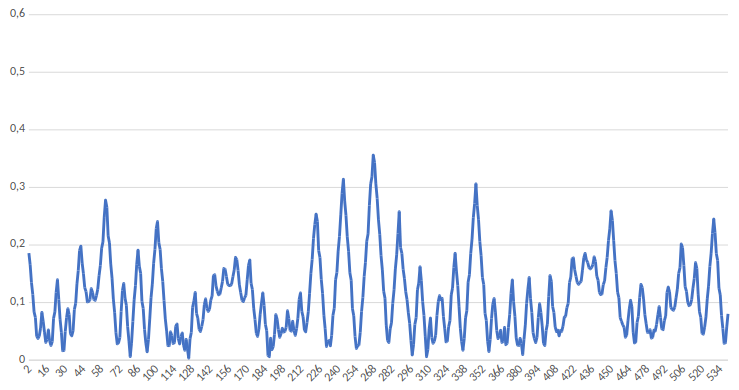
\includegraphics[width=0.5\textwidth]{imag/IMG38.png}}
  \subfloat[Piloto Antiguo]{
   \label{f:Piloto Antiguo}
    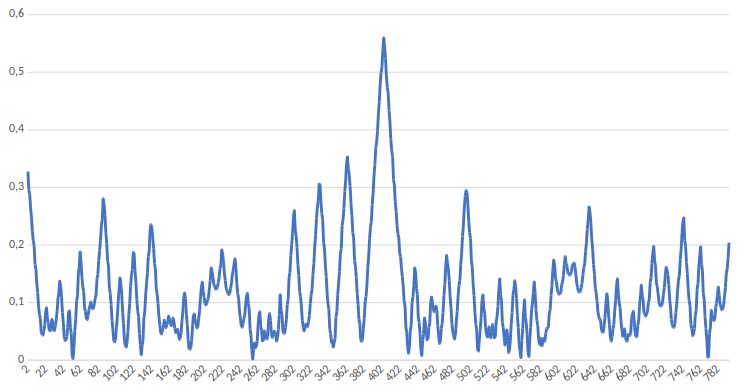
\includegraphics[width=0.5\textwidth]{imag/IMG39.png}} 
 \caption{Comparación del error entre ambos pilotos en ruta compleja.}
 \label{f:Comparativa del error compleja.}
\end{figure} 

\hspace{1cm} Para poder observar mejor el error en cuanto a distancia sobre la ruta deseada del pilotaje, sometimos los pilotos a una trayectoria con curvas mucho más pronunciadas y con cambios de altitud bruscos. Esta trayectoria se puede observar en la imagen \ref{fig:Ruta compleja en trayectoria.} donde tenemos la trayectoria deseada en verde, el piloto nuevo en azul y el piloto antiguo en rojo. En esta imagen sí que se ve con mayor claridad como el piloto nuevo se ajusta mucho más a la ruta deseada, se corrobora con los datos de las gráficas \ref{f:Comparativa del error compleja.} en los cuales el error medio del piloto nuevo es de 0.106m y el error máximo es de 0.356m mientras que el error medio del piloto antiguo es de 0.119m con un error máximo de 0.559m. A su vez el nuevo piloto tarda 59.85 segundos en realizar la ruta mientras que el antiguo lo hace en 84.82 segundos reduciendo en este caso el tiempo de ruta en un 29.44\% por lo que en rutas complejas el nuevo piloto se desenvuelve mejor que el antiguo en todos los aspectos.

\section{Pruebas integrales del sistema}
\hspace{1cm} Una vez conseguido que los componentes por separado funcionasen correctamente y demostrando que hemos conseguido errores mínimos en su comportamiento, se integraron ambos componentes conjuntamente y se realizaron las pruebas finales del sistema. Pese a la complejidad de unir los dos componentes ya que cada uno utilizaba unas velocidades máximas del drone y unos datos diferentes de posicionamiento, cuando se consiguió combinar y al haber realizado las pruebas por separado con buenos resultados, se esperaba que al unirlos los resultados siguiesen siendo óptimos. Esto se corroboro con los experimentos tanto de la ruta por puntos \ref{fig:Prueba integral de ruta por puntos.} donde tenemos en verde la ruta deseada, en rojo la posición estimada y en azul la ruta realizada, como de la ruta por trayectorias \ref{fig:Prueba integral de ruta por trayectoria.} que analizaremos a continuación con más detalle ya que es el experimento final más complejo, aun así en ambas se ve como el drone seguía la ruta de forma estable y con un margen de error prácticamente nulo, siempre y cuando estén a la vista del vehículo balizas AprilTags. 

\begin{figure}[H]
	\begin{center}
		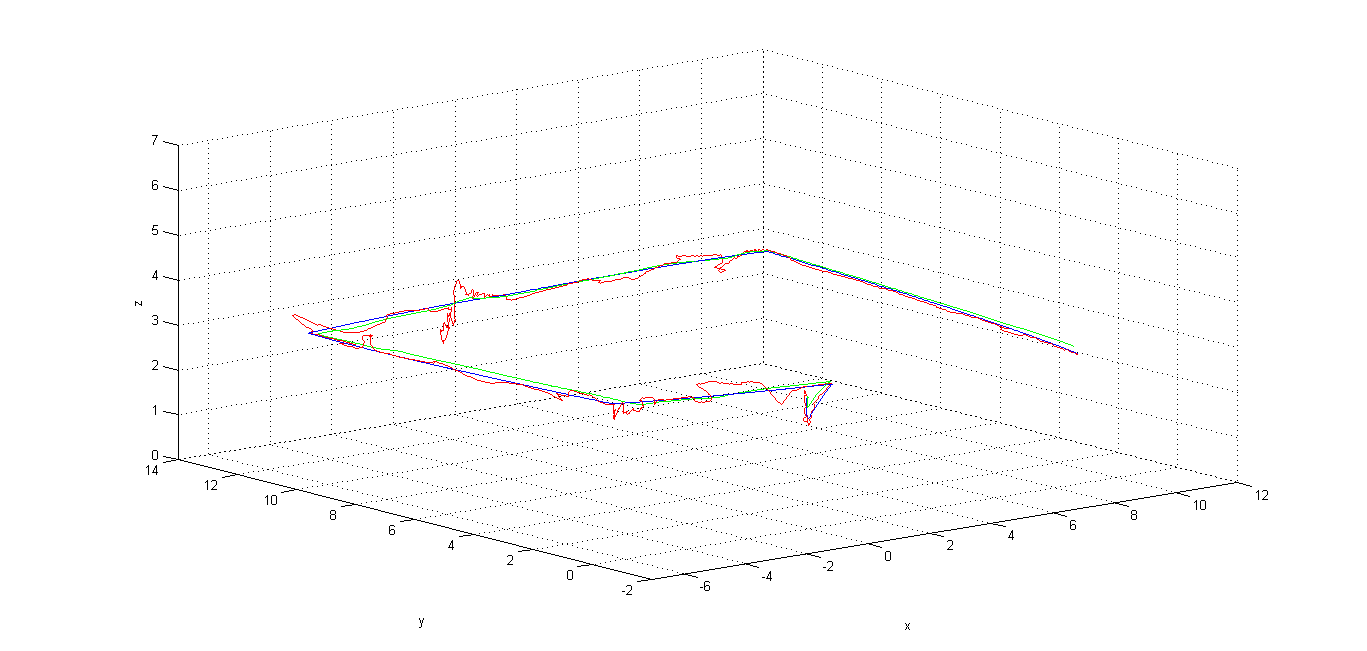
\includegraphics[width=1\textwidth]{imag/IMG42.png}
				\caption{Prueba integral de ruta por puntos.}
		\label{fig:Prueba integral de ruta por puntos.}	
	\end{center}
\end{figure}

\begin{figure}[H]
	\begin{center}
		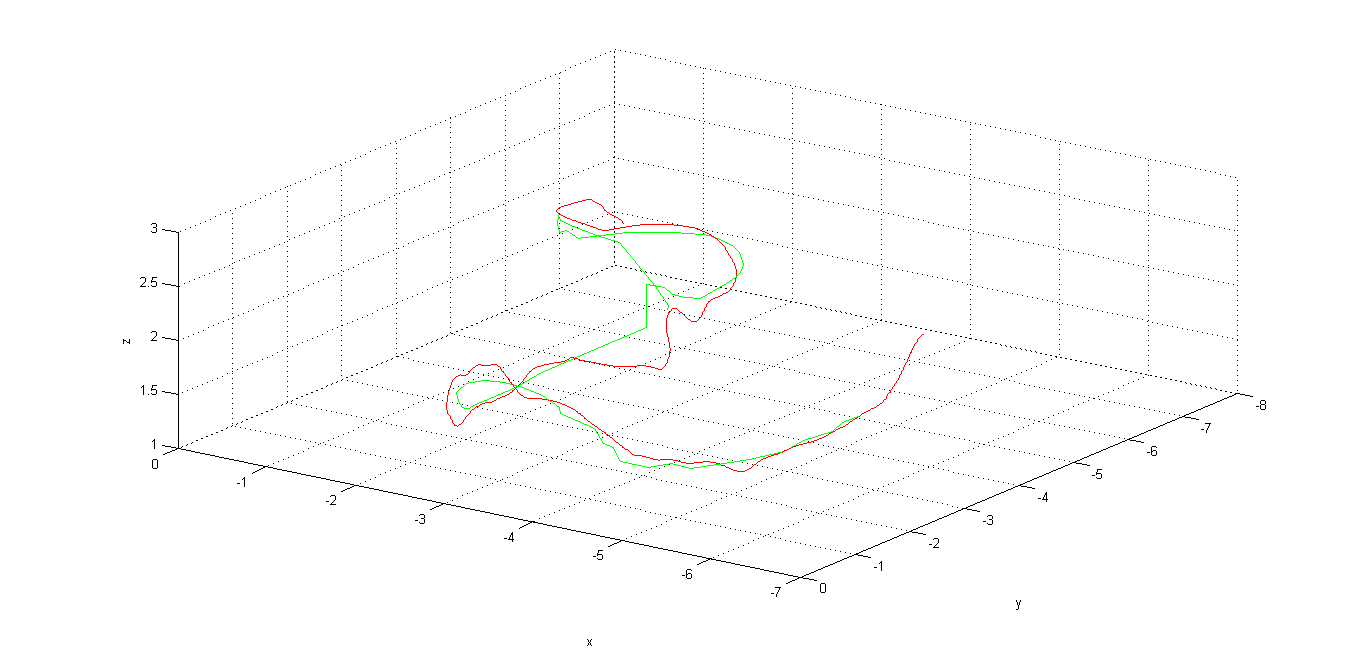
\includegraphics[width=1\textwidth]{imag/IMG43.png}
				\caption{Prueba integral de ruta por trayectoria.}
		\label{fig:Prueba integral de ruta por trayectoria.}	
	\end{center}
\end{figure}

\hspace{1cm} Para la realización del experimento final decidimos utilizar una trayectoria compleja con curvas cerradas y saltos de altura, así comprobar la integridad y el error de la aplicación para cualquier situación. En la imagen \ref{fig:Prueba integral de ruta por trayectoria.} se observa la ruta deseada en verde y la ruta realizada en rojo. A primera vista no se aprecian errores demasiado elevados, por lo que calculamos la gráfica \ref{fig:Error de distancia final.} para obtener los datos numéricos reales. De esta extraemos que el error medio de distancia en una ruta compleja es de 0.128m con un error máximo de 0.563m, debido a que el reconocimiento de las balizas no se puede realizas a velocidades elevadas el tiempo de ruta ha aumentado a los 109.5 segundos.

\begin{figure}[H]
	\begin{center}
		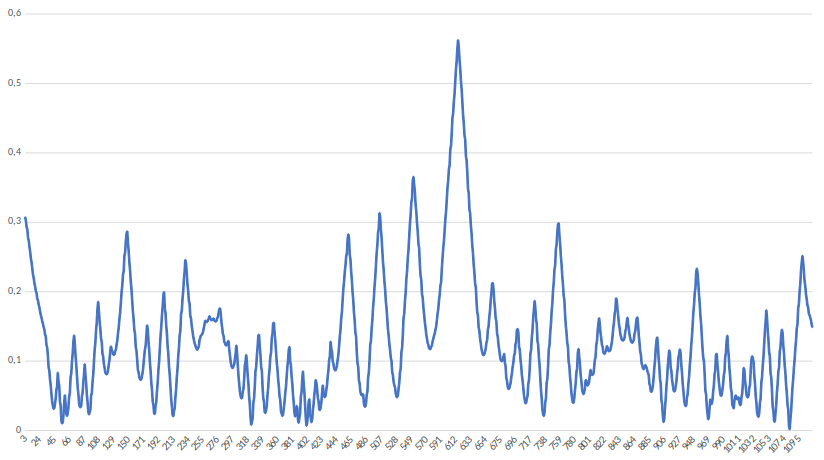
\includegraphics[width=1\textwidth]{imag/IMG44.png}
				\caption{Error de distancia a la ruta deseada en la prueba integral del sistema}
		\label{fig:Error de distancia final.}	
	\end{center}
\end{figure}

\hspace{1cm} Por último anotar que el piloto cuenta con un margen de error de 15cm, lo que permite al vehículo realizar maniobras más amplias para evitar giros abruptos y así conseguir estabilidad durante toda la ruta. También destacar las nuevas funcionalidades que lo preparan para el mundo real que son la función en el pilotaje de que cuando un punto no lo puede alcanzar correctamente por una limitación en sus movimientos aterrice y no se quede infinitamente dando vueltas sobre este punto sin probabilidad de éxito, y la nueva función basada en el nuevo Slam-VisualMarkers de Ros utilizando la constante del número de balizas en vista, creada explícitamente para ello, esta permite que en el momento que está 2 segundos sin ver ninguna AprilTag el drone cese en su intento de seguir la ruta ya que no está recibiendo una localización real y que gire en círculos cada vez mayores en torno al último punto para así encontrar la baliza anterior y poder volver a localizarse y seguir la ruta, si no lo consigue aterrizara para evitar que intente conseguir una autolocalización errónea y se pierda en su intento de seguir la ruta deseada.